
\par
W celu przeglądania i porównywania należy posiadać narzędzie do wyświetlenia w sposób poprawny, najlepiej jednym i tym samym programem.
%\par
%Standard \DICOM pozwala na odczytanie badania i wyświetlanie go w postaci obrazów radiologicznych, scyntygraficznych, itd.

\subsection{Przeglądarki obrazów}

Przeglądarki obrazów to programy należące do kategorii przeglądarki plików.
Zwykłe przeglądarki obrazów takich jak jpg, png lub gif wyświetlają obraz w takiej postaci jakiej jest zapisany, najpierw przeprowadzając dekompresję tego obrazu.
W przypadku obrazów medycznych najczęściej nie mamy do czynienia z danymi reprezentującymi kolory w spektrum światła widzialnego.
Przeglądarka obrazów \DICOM musi wygenerować kolorowy obraz z danych na podstawie parametrów obrazu.

\subsection{Funkcje przeglądarki obrazów}

\subsubsection{Obsługa wielu formatów danych}

Standard \DICOM przewidział możliwość zapisania wielu typów danych w różnych formatach, nie tylko obrazów, ale też nagrań nagrań audio i tekstów.
Przeglądarka obrazów \DICOM może mieć możliwość od czytania, wyświetlenia lub odsłuchania danych.

\subsubsection{Podstawowe operacje na obrazie}

\begin{itemize}
    \item Skalowanie lub powiększenie, czyli możliwość powiększenia lub zmniejszenia wyświetlanego obrazu o pewny współczynnik skalujący.

    \item Przesuwanie \fromEng{pan}, czyli możliwość przesuwania obrazu o dowolny wektor.
          Jest to przydatne, gdy powiększymy obraz do takiego stopnia, że nie będzie mieścił się na ekranie lub w okienku programu.

    \item Lupa, skalowanie miejscowe.
          Jest to możliwość miejscowego powiększenia obrazu.
          Przykład użycia takiego narzędzia znajduje się na rysunku \ref{fig:wyswietlanie001}.

          \begin{figure}[!htbp]
              \centering
              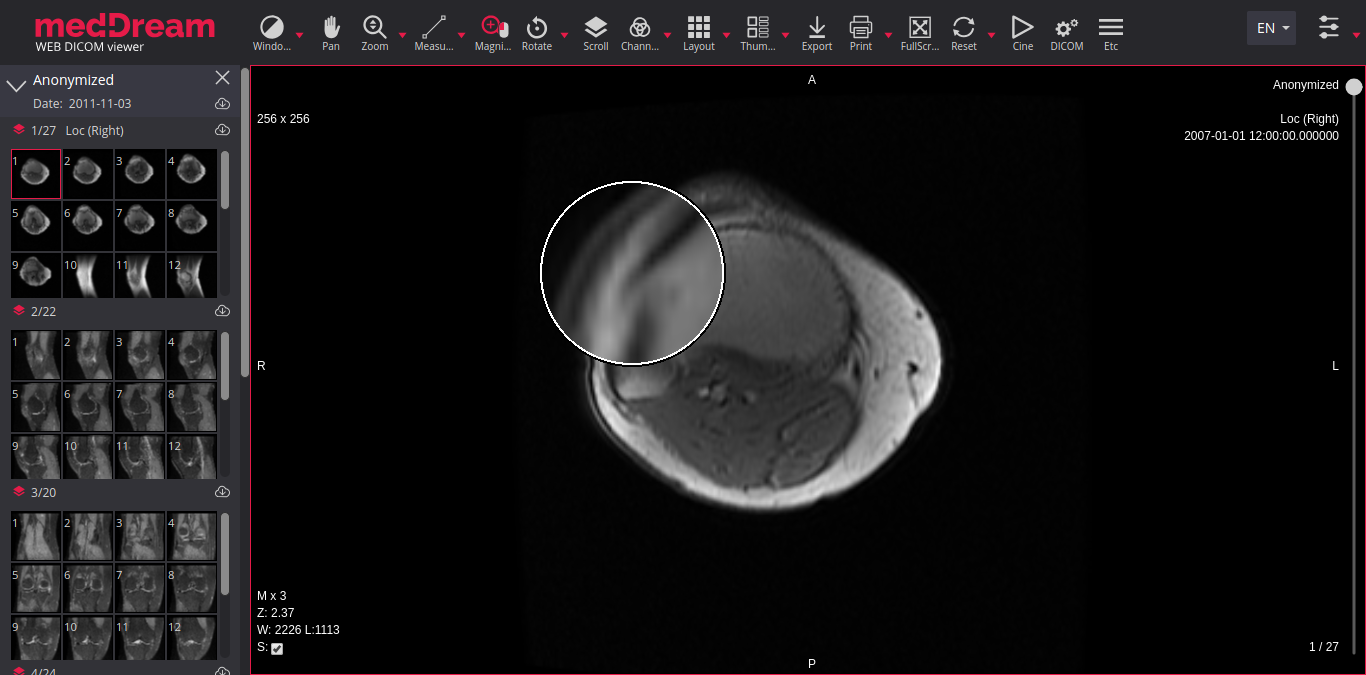
\includegraphics[width=\textwidth]{img/wyswietlanie001.png}
              \caption{Narzędzie Lupa w przeglądarce \href{https://www.softneta.com/products/meddream-dicom-viewer/}{MedDream DICOM Viewer}. Zdjęcie użyte za zgodą \href{https://www.softneta.com/}{Softneta UAB}.}
              \label{fig:wyswietlanie001}
          \end{figure}

    \item Rotacja i odbicia lustrzane, czyli możliwość obrócenia obrazu o zadany kąt oraz możliwość uzyskania odbicia lustrzanego obrazu w dwóch osiach X i Y.

\end{itemize}

\subsubsection{Analiza parametrów w celu lepszej informacji}

\begin{itemize}
    \item Okienkowanie.
          Termin odnosi się do używania funkcji okna cyfrowego w celu zamiany obrazu danych na obraz monochromatyczny możliwy do wyświetlenia.%TOASK
          Okienkowanie jest szczegółowo opisane w sekcji \ref{sec:algorithm-pixmap-monochrome} wraz z generowaniem obrazu monochromatycznego.

    \item Maski \fromEng{overlay}.
          Jest to możliwość nałożenia maski, elementu, który będzie przysłaniał fragment obrazu w celu lepszej wizualizacji bądź ukrycie mało wartościowych obiektów, np. tła.
          Standard \DICOM umożliwia nałożenie wielu masek na jeden obraz.
\end{itemize}

\subsubsection{Obsługa wielu plików}

\begin{itemize}

    \item Obsługa DICOMDIR.
          Jest to możliwość wczytania pliku DICOMDIR i wyświetlenie struktury serii badań.
          Plik DICOMDIR to wiele zindeksowanych plików zawierający ich zbiór elementów danych, bez obrazów.

    \item Wczytanie wielu plików i ich połączenie w formie filmu, czyli możliwość wczytania wielu plików z tej samej serii, ułożenia ich według pozycji geometrycznej i wyświetlenia ich jako film.
          Innymi słowy jest periodyczna podmiana obrazu na obraz następny w serii.

    \item Wyświetlanie wielu obrazów jednocześnie.
          Jest to możliwość wyświetlenia kilku obrazów w postaci tabelki, w której każda komórka była by innym obrazem.

          Przykład wyświetlenia wielu obrazów na raz w jednym oknie znajduje się na rysunku \ref{fig:dicomviewer001}

          \begin{figure}[!htbp]
              \centering
              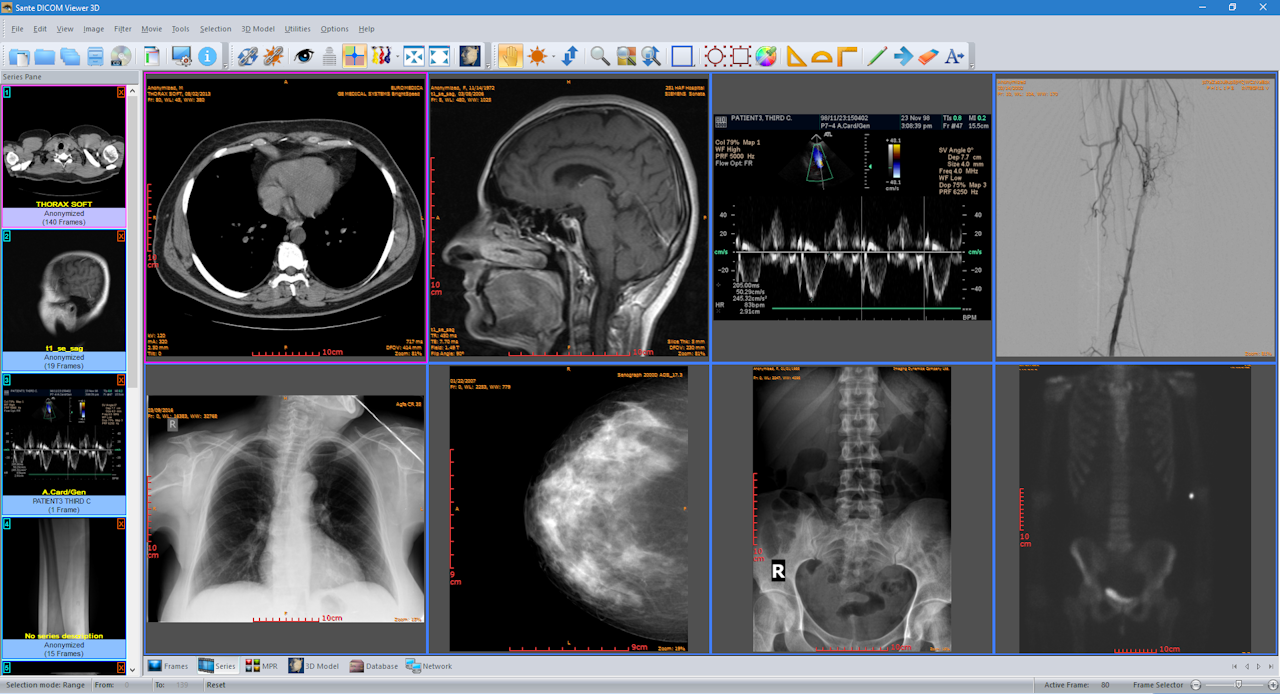
\includegraphics[width=\textwidth]{img/dicom-viewer-001.png}
              \caption{Wyświetlenie wielu obrazów na raz w jednym oknie w przeglądarce \href{https://www.santesoft.com/win/sante-dicom-viewer-3d-pro/sante-dicom-viewer-3d-pro.html}{Sante DICOM Viewer 3D Pro}. Zdjęcie użyte za zgodą \href{https://www.santesoft.com/}{Santesoft}.}
              \label{fig:dicomviewer001}
          \end{figure}
\end{itemize}

\subsubsection{Generowanie obrazów woliumetrcznych}

Jeżeli mamy do dyspozycji wiele obrazów tomograficznych o znanych parametrach to możemy wczytać je, posegregować a następnie wygenerować trójwymiarowy obiekt, który wyświetlany jest ekranie komputera za pomocą trójwymiarowej grafiki komputerowej.

Przykład takiego obrazu znajduje się na rysunku \ref{fig:dicomviewer002}.

\begin{figure}[!htbp]
    \centering
    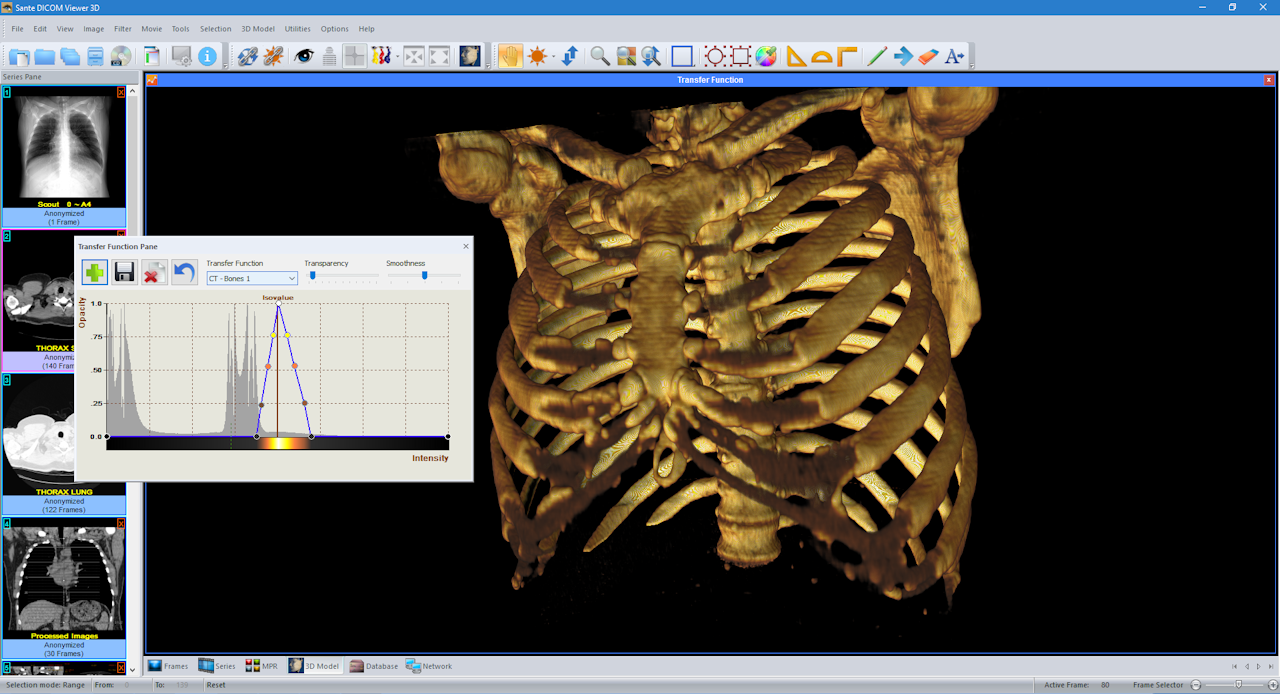
\includegraphics[width=\textwidth]{img/dicom-viewer-002.png}
    \caption{Generowanie obrazów 3D z wielu obrazów tomograficznych w przeglądarce \href{https://www.santesoft.com/win/sante-dicom-viewer-3d-pro/sante-dicom-viewer-3d-pro.html}{Sante DICOM Viewer 3D Pro}}
    \label{fig:dicomviewer002}
\end{figure}

\subsubsection{Analiza i przetwarznie danych}

\begin{itemize}
    \item Histogram, czyli możliwość wygenerowania histogramu obrazu.

          Histogram to wykres przedstawiający dystrybucje wartości numerycznych obrazu.

    \item Mierzenie i wykonywanie pomiarów.
          Pozwala na określenie odległości pomiędzy dwoma punktami przez lekarza lub zmierzenie wielkości/pola zadanego kształtu.

    \item Rekonstrukcja wielopłaszczyznowa.
          Obrazy tomograficzne przedstawiają przekroje.
          Jeżeli parametry wielkości woksela są dostępne to istnieje możliwość wygenerowania nowego obrazu, który byłby przekrojem poprzecznym.

          Przykład generowania rekonstrukcji wielopłaszczyznowej jest pokazany na rysunku \ref{fig:dicomviewer003}

          \begin{figure}[!htbp]
              \centering
              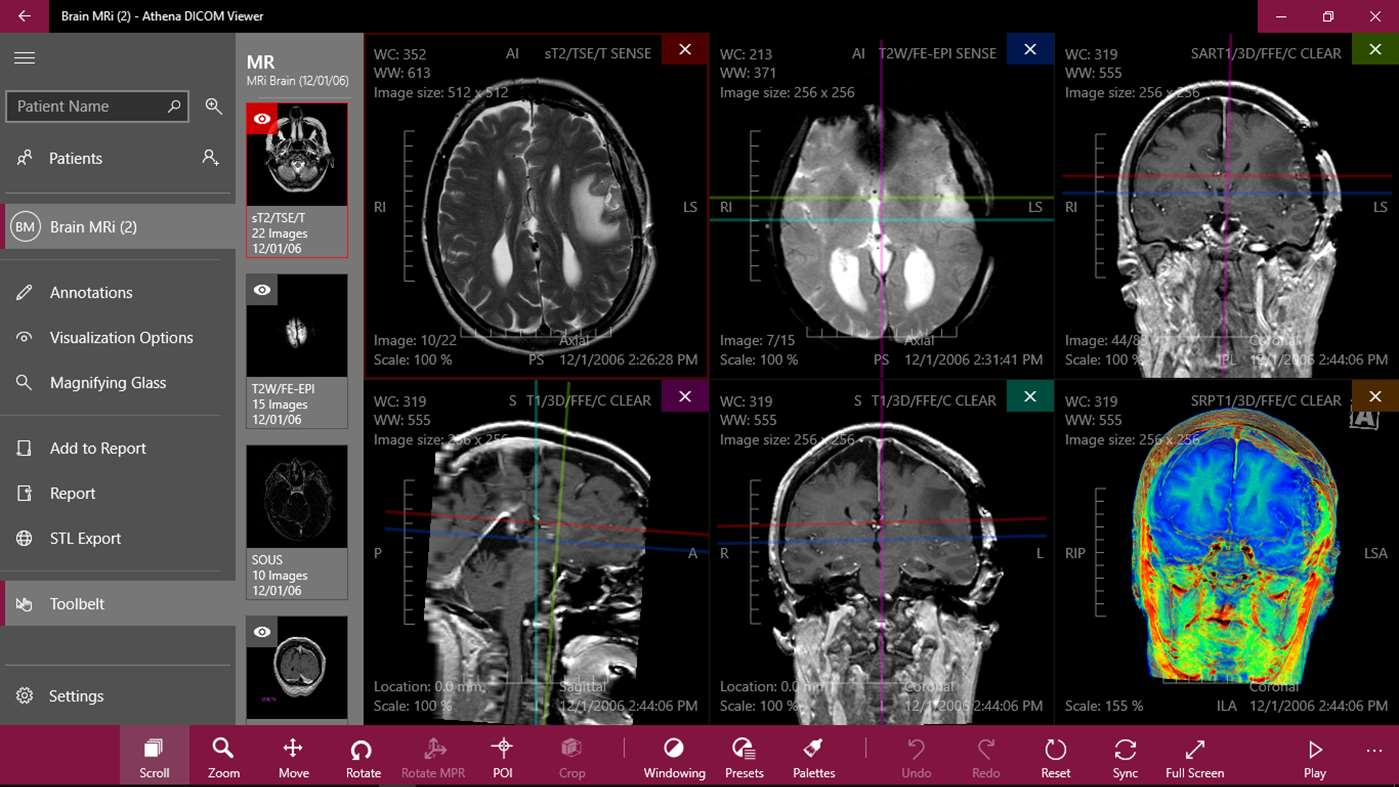
\includegraphics[width=\textwidth]{img/dicom-viewer-003.jpeg}
              \caption{Rekonstrukcji wielopłaszczyznowej w przeglądarce \href{https://athenadicomviewer.com/}{Athena DICOM Viewer}. Zdjęcie użyte za zgodą \href{https://medicalharbour.com/}{Medical Harbour}.}
              \label{fig:dicomviewer003}
          \end{figure}
\end{itemize}

\subsubsection{Edycja danych}

\begin{itemize}
    \item Dodawanie nowych obiektów.
          Pozwala na rysowanie, dodawanie figur geometrycznych lub tekstu przez lekarza i zapis tych informacji w pliku \DICOM.
          Chodzi tu głównie o szkice i notatki tworzone podczas analizy obrazu przez personel medyczny.

    \item Edycja parametrów oraz anonimizacja danych.
          Jest to możliwość edycji parametrów w pliku \DICOM w różnych celach.
          Funkcja jest używana do usuwania danych osobowych pacjenta w celu późniejszej publikacji obrazu.

\end{itemize}

\subsection{Kryteria porównywania przeglądarek obrazów}

Porównanie aplikacji posiadających tak wiele parametrów jak przeglądarki \DICOM jest bardzo skomplikowanym procesem.
Dlatego wyróżniono 26 kryteriów do ich porównywania w postaci logicznej: „tak” lub „nie”, podzielonych na 5 grup, platformy, interfejsu, wsparcia, obrazowania dwu i trójwymiarowego \cite{SurveyofDICOMViewer}.
Kryteria te w jasny sposób pozwalają na ocenę praktycznych aspektów użytkowania przeglądarki.

\subsubsection{Platforma}

Grupa platforma zawiera kryterium samodzielności.
Aplikacje samodzielne są zaprojektowane tak, aby nie wymagały żadnego dodatkowego sprzętu fizycznego bądź infrastruktury do poprawnego działania.
Rozwiązania sieciowe określają czy aplikacja jest usługą sieciową i czy można z aplikacji korzystać jak ze strony WWW.
Aplikacje są wieloplatformowe, czyli mają możliwość uruchomienia ich na różnych systemach operacyjnych Linux/MacOS/Windows oraz możliwość używania ich na urządzeniach mobilnych takich jak telefon.

\subsubsection{Interfejs}

Przeglądarka powinna mieć możliwość komunikacji z interfejsami innych systemów.
Podstawowe interfejsy sieciowe to: C-STORE SCP DICOM C-STORE, C-STORE SCU, Query-Retrieve, WADO, Parameter Transfer.

\subsubsection{Wsparcie techniczne}

Aplikacja powinna mieć dostępną pisemną dokumentację oprogramowania (np. podręczniki lub strony internetowej), wsparcie przez pocztę internetową, możliwość porozumienia się z twórcą lub opiekunem oprogramowania.
Forum, możliwość pytania się społeczności o opinie i ich wymiana.
Wiki, strona internetowa w formacie Wikipedii dostępna dla użytkownika.

\subsubsection{Obrazowanie dwuwymiarowe}

Przewijanie\fromEng{scroll}, proces wyświetlania obrazów, można poprawić dzięki zmniejszeniu interakcji z klawiaturą oraz myszką. Można to osiągnąć na przykład, oferując możliwość przejścia do następnego lub poprzedniego obrazu przez przesunięcie kółkiem myszy lub używając przycisków góra/dół na klawiaturze.
Metadane, przeglądania powinna obejmować analizowanie i wyświetlanie metadanych obiektów DICOM, powinna obejmować wyświetlanie rozdzielczości obrazu, badanie (np. identyfikator podmiotu) oraz znaczniki DICOM specyficzne dla dostawcy (np. specjalne ustawienie urządzenia rejestrującego).
Warstwa informacyjna, najważniejsze informacje powinny powinny być wizualizowane w oknie wyświetlacza jako nakładka na obraz.
Na przykład aktualna pozycja lub nazwa podmiotu wykonującego badanie.
Okienkowanie to sposób zamiany danych na skale szarości, okienkowanie jest opisane w sekcji \ref{sec:algorithm-pixmap-monochrome}.
Pseudo-kolorowanie obrazu, tabele (LUT, \fromEng{LookUpTable}) odwzorowujące szare wartości obrazu na pseudo-kolory.
Histogram wizualizuje wystąpienia i rozkład wartości kolorów na obrazach, pozwalają opisywać istotne cechy obrazu
Wymiarowanie, możliwości rysowania bądź zaznaczania linii lub innych kształtów do analizy i wyznaczania odległości w jednostkach długości na obrazie.
Jest to możliwe gdyż nagłówki pliku DICOM zawierają parametry sprzętowe urządzenia (np. ilość pikseli na centymetr).
Adnotacje(opisy), które były wytworzone przez personel medyczny powinny być zapisywane w odpowiedni sposób w pliku.

\subsubsection{Obrazowanie trójwymiarowe}

Rekonstrukcja wtórna, zwykle dane dotyczące objętości medycznej są gromadzone wzdłuż jednej osi ciała (np. poprzecznej).
W wielu przypadkach ważne jest przeglądanie danych w innych kierunkach (np. strzałkowych lub czołowych), aby poprawić wizualizację niektórych struktur.
W tym celu należy zapewnić funkcjonalność rekonstrukcji osi pomocniczej na podstawie kierunku pierwotnego.
Plastry objętości kostki(\fromEng{Slice Cube Volume}), przekroje mogą być lepiej wyświetlane w określonej pozycji.
Funkcjonalność kostki plasterka umożliwia niezależną regulację położenia różnych osi wycinków (np. poprzecznych, strzałkowych lub czołowych) w modelu objętościowym.
Podczas tego przekroje są pokazane w osobnym oknie.
Renderowanie objętościowe – dane obrazu 3D są bezpośrednio wizualizowane jako objętość.
Użytkownik może wchodzić w interakcje z woluminem poprzez obracanie lub skalowanie.
Transfer Function(nie znam polskiej nazwy), służy do odwzorowania wartości szarości obrazów wokseli na wartości krycia typów tkanek (np. kości). Struktury obrazu pasujące do wzorców szarych wartości są podświetlone. Niewykorzystane szare wartości są wyświetlane jako
przezroczyste. Specyficzne struktury stają się lepiej widoczne.
Generowanie powierzchni, dzięki różnym algorytmom można generować powierzchnie w postaci wokselów. Reprezentacje powierzchni można również zastosować do poprawy wizualizacji niektórych struktur obrazu.